\documentclass[11pt]{article}

% These are some useful packages, but feel free to add more!
\usepackage{amsmath, amsfonts, amsthm, amssymb}  % Math Symbols
\usepackage[utf8x]{inputenc}
\usepackage{fullpage}
\usepackage{graphicx}
\usepackage{multicol}
\usepackage[table]{xcolor}

\title{CSE 301: Lab 1} 
\author{John Ezra See} %%TODO: Add Your Name
\begin{document}

\maketitle
\section*{Introduction}
    You can address me by my first name, John. I go by he/him. I am a junior who is planning to graduate in December 2025. I am mostly looking forward to building upon the materials from CS 151 and seeing how everything connects with each other.
\hspace{10 cm}

\section*{Labmates}
\begin{itemize}
    \item Joel Lau Arrieta
    \item Don Nguyen
    \item Angelo Mustafa
\end{itemize}
\hspace{10 cm}

\section*{Five of my Favorite Things}
\begin{enumerate}
    \item CS \\
    \item Piano \\
    \item Good Music \\
    \item Korean Fried Chicken \\
    \item Friends \\
\end{enumerate}
\hspace{10 cm}

\section* {Animal Picture}
\begin{figure}[ht]
\centering 
% https://www.thoughtco.com/thmb/JT-Zx0vKKPlgsj5NmVk3fjZEs5k=/1500x0/filters:no_upscale():max_bytes(150000):strip_icc()/GettyImages-826128004-6cb21c0037424480b047a648e294e669.jpg
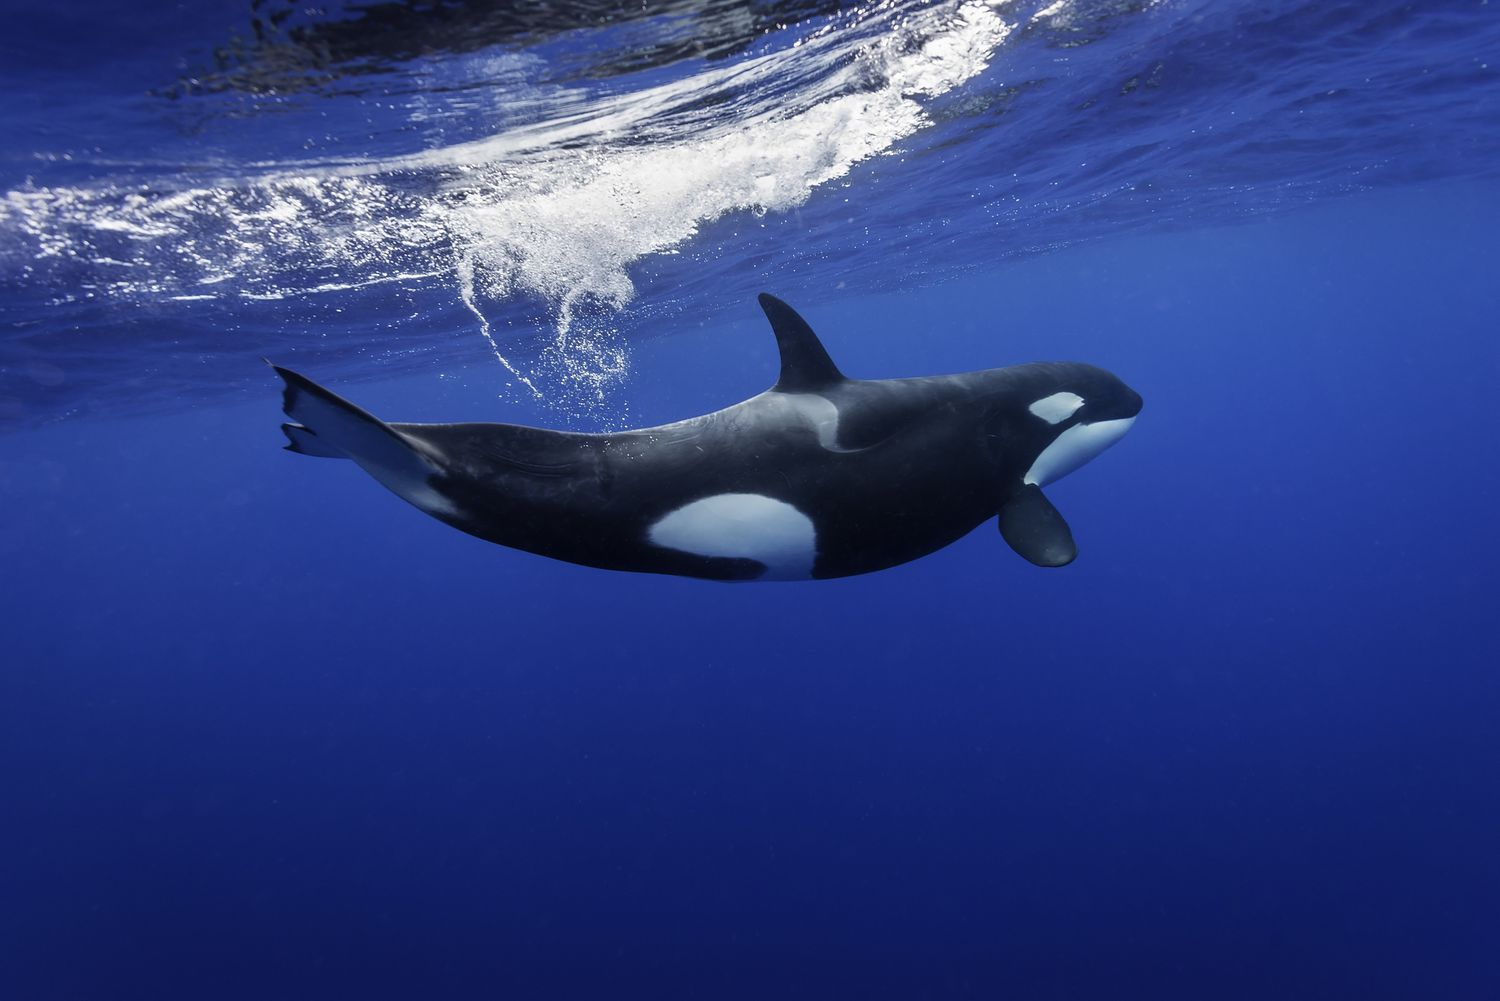
\includegraphics[width=0.5\textwidth, height=0.2\textheight, keepaspectratio, origin=c]{orca.jpg}
\caption{This is a picture of my favorite sea animal.}
\end{figure}

\hspace{10 cm}

\section*{Symbol Practice}
%% A ∪ B = {x : x ∈ A ∨ x ∈ B}
\[A \cup B = \{x : x \in A \lor x \in B\}\]
\hspace{10 cm}
\end{document}